\section{Model selection}

We tried severall models: linear regression, K-nearest neightbors (KNN), multi-layer perceptron and a random forest. For each model except the linear regression, we choosed to tweak severall well chosen hyperparameters and used a searching algorithm along with cross-validation to find the best hyperparameters for each model. A common searching algorithm is \textit{Grid Search} that will test every possible combination of hyperparameters. However, it can be computationaly intensive if the search space is wide which is often the case since we don't want to miss the optimal parameters. Another approach is to use \textit{Random Search}. With this approach, we can also draw hyperparameter configurations from distributions besides discrete sets and the random search will randomly select a combination of hyperparameters among the ones defined instead of doing an exhaustive search. It allows to explore a wide range of hyperparameter configurations with time-efficiency. Looking at the result of the random search, we can identify the area where the results are promising, tighten our ranges and perform a random search again. Although this algorithm being less computationaly intensive, it can be time consuming of running and running again the random search to find the best set of hyperparameters. A third approach and the one we tried in this project is to perform a \textit{Bayesian Search} which is basically similar to random search but...

\begin{figure}[H]
	\centering
	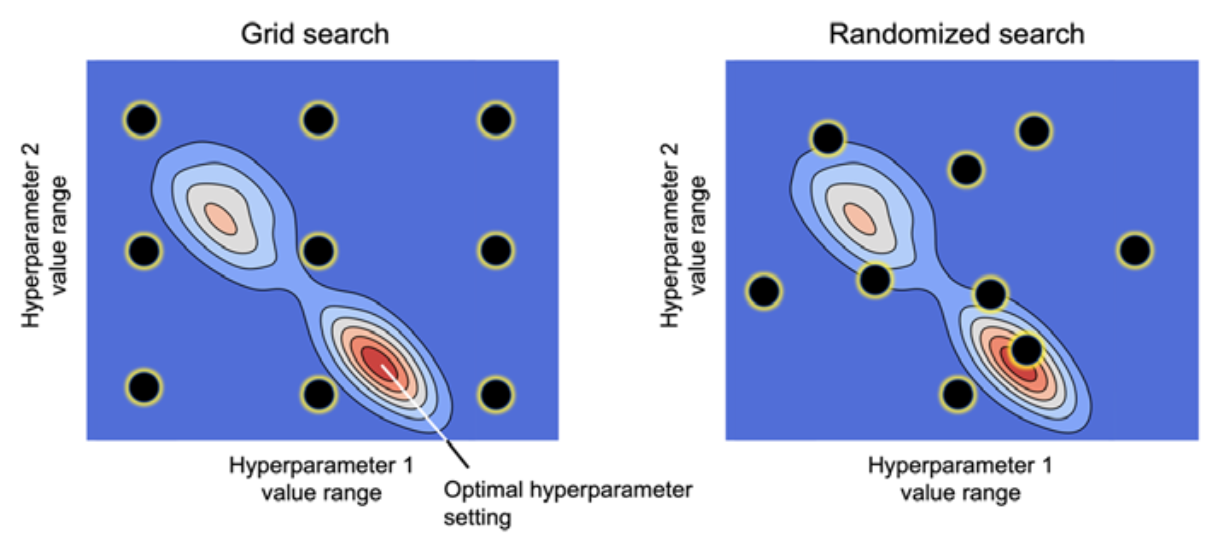
\includegraphics{figures/grid_search_vs_random_search.png}
	\caption{Comparison of grid search and randomized for sampling $9$ different hyperparameter configurations}
	\label{fig:gridsearch_vs_randomsearch}
\end{figure}